\cia \vspace{-2cm}
\section{$\cos\theta^*$ cuts}
In Section \ref{sec:cmsystcomp} it was mentioned that the Invariant method of
calculating  $\cos\theta^*$ yelded unphysical results at $\cos\theta^*$ extremes
due to the smearing introduced by the CLAS detectors and reconstruction software and possibly 
to the rescattering of the proton in the torus coils.
In order to study this possible cause of systematic errors, different cuts have been applied
to  $\cos\theta^*$.  The values are shown in  Table \ref{tab:costheta_cuts}.




\begin{table}[h]
 \begin{center}
  \begin{tabular}{c  c}
    & \\
    min &  max   \\ 
    & \\
    \hline
    & \\
    -1     & 1  \\
    -0.95  & 0.95 \\ 
    -0.90  & 0.90  \\
    -0.85  & 0.85 \\
  \end{tabular}
 \end{center} 
 \caption{$\cos\theta^*$  cuts}
 \label{tab:costheta_cuts}
\end{table}


The cuts are illustrated in \F{fig:ccuts}.

\begin{figure}[h]
 \begin{center}
  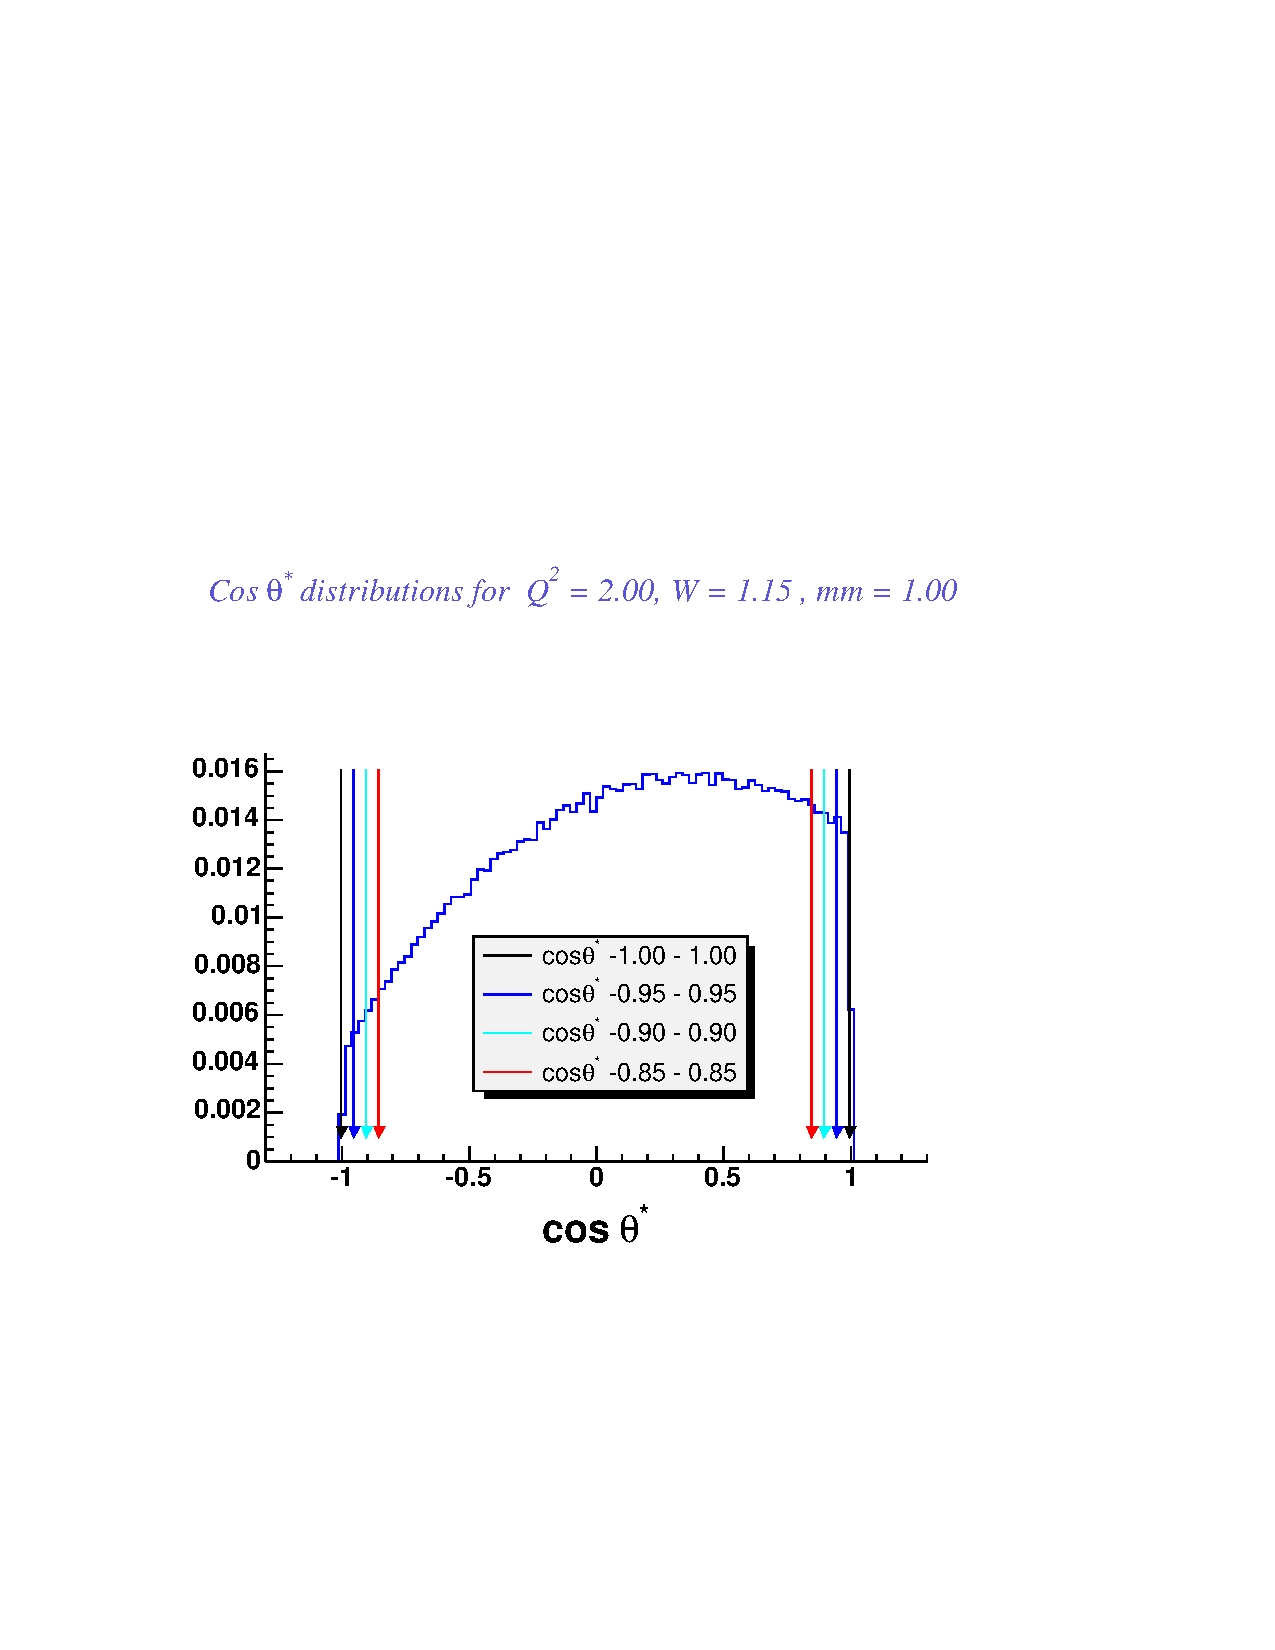
\includegraphics[width = 11cm, bb = 80 150 500 520]{systematics/img/ccuts}
  \caption{ Different cuts for $\cos\theta^*$ as shown in Table \ref{tab:costheta_cuts}. 
            The distribution comes from the MonteCarlo reconstructed events, and it's normalized to $1$.}
  \label{fig:ccuts}
 \end{center}
\end{figure} 


The variation of the ratios $R_{EM}$ and $R_{SM}$ for the first and second cut is illustrated in 
\F{fig:ratios_cc_syst}.
\begin{figure}[h]
 \begin{center}
  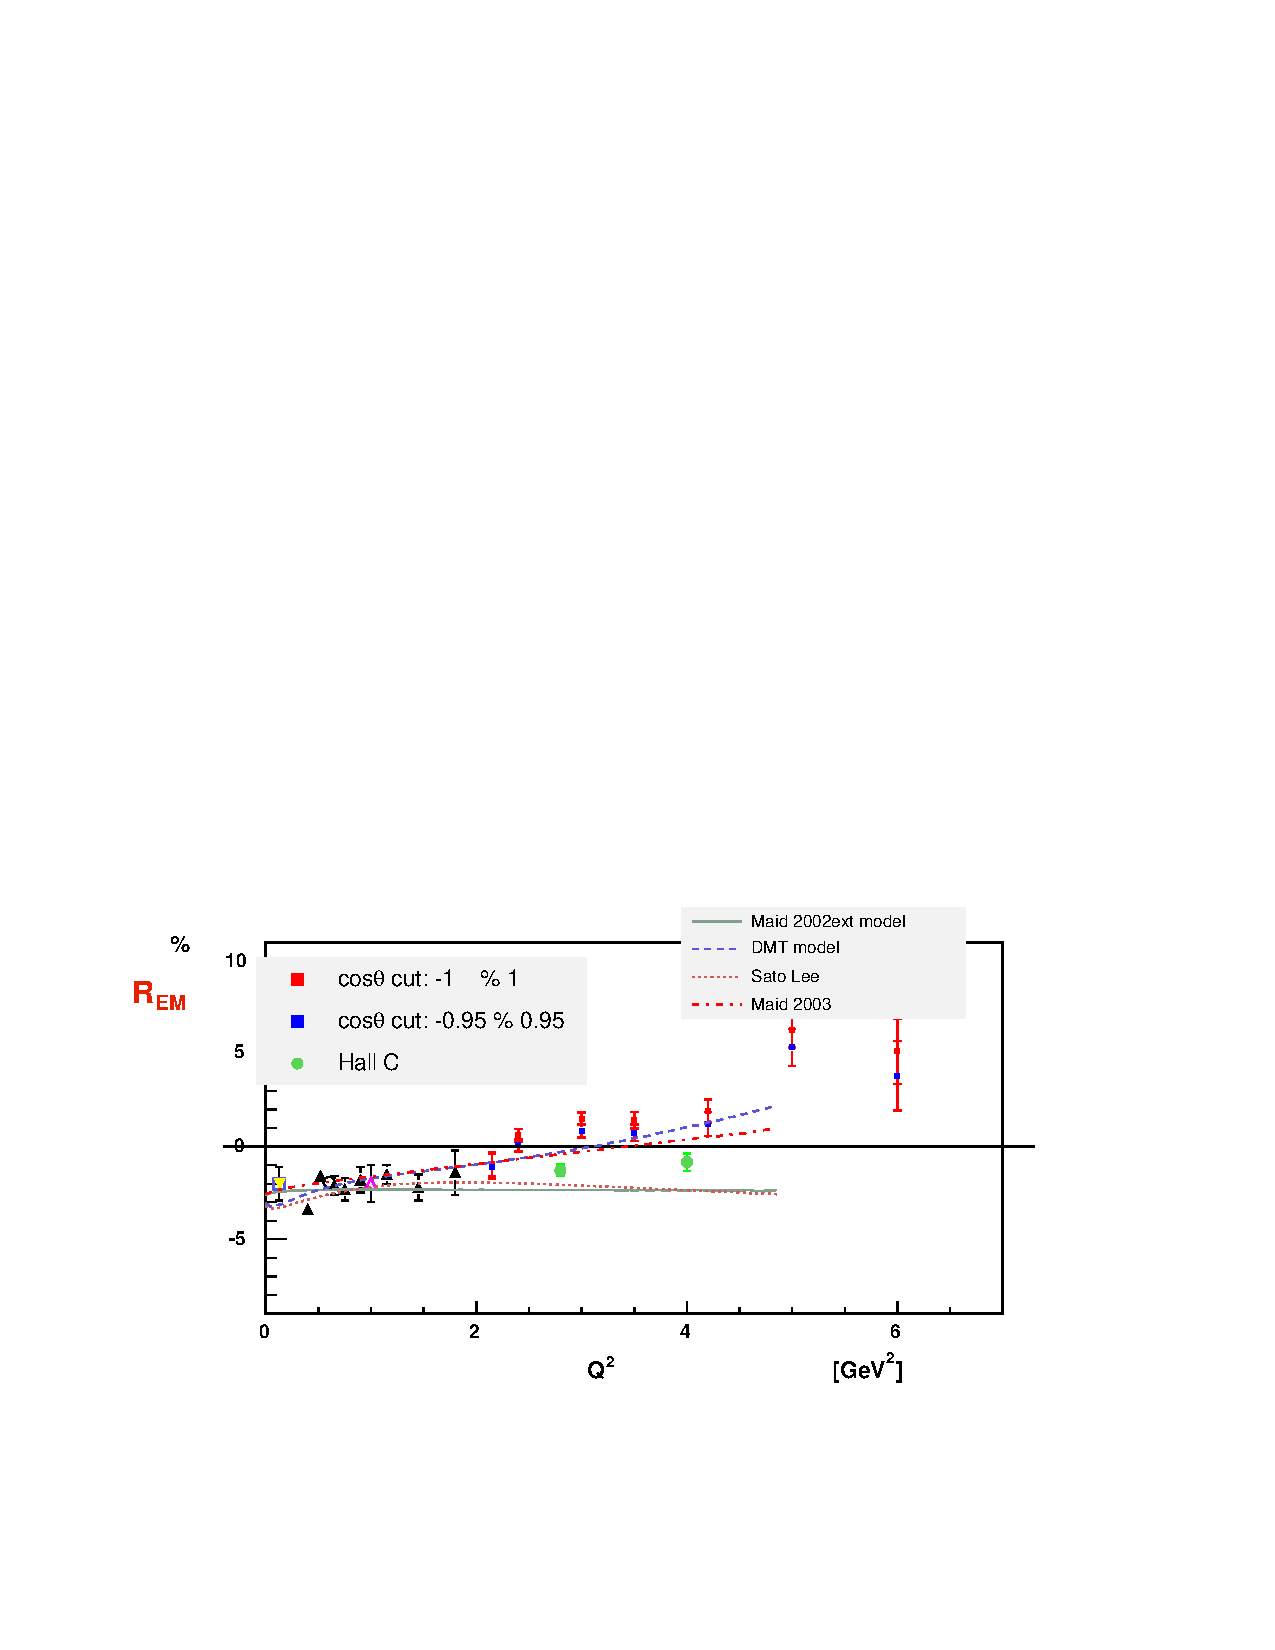
\includegraphics[width = 12cm, bb = 50 120 540 440]{systematics/img/rem_ccsyst}
  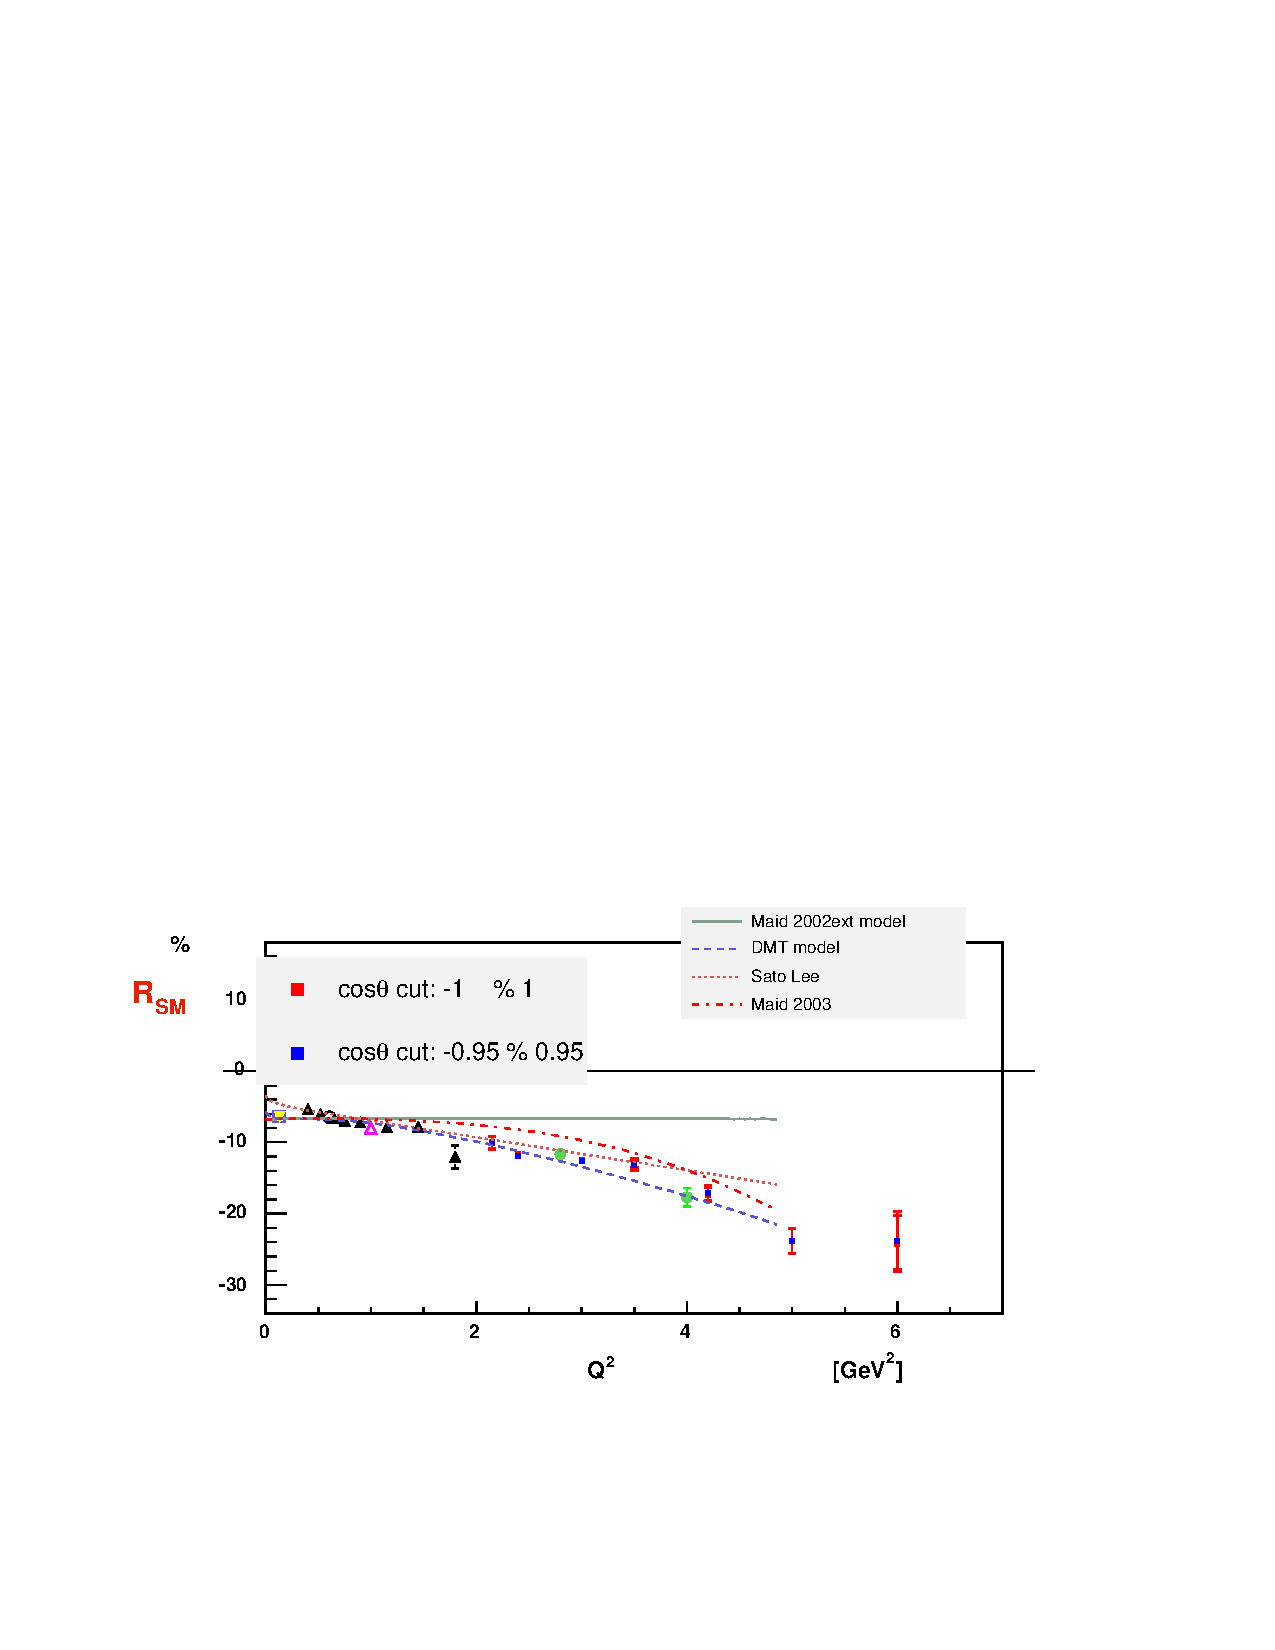
\includegraphics[width = 12cm, bb = 50 100 540 440]{systematics/img/rsm_ccsyst}
  \caption{ Variation of the ratios $R_{EM}$ (top) and $R_{SM}$ (bottom) for the $\cos\theta^*$ cuts:
           $-1 < \cos\theta^* < 1$ and  $-0.95 < \cos\theta^* < 0.95$. }
  \label{fig:ratios_cc_syst}
 \end{center}
\end{figure} 


















